\documentclass[10pt]{article}
\usepackage[margin=0.85in]{geometry}
\usepackage{graphicx,booktabs,amsmath,amssymb,amsthm,hyperref,enumitem,xcolor}
\hypersetup{colorlinks,linkcolor=blue!50!black,citecolor=blue!50!black,urlcolor=blue!50!black}
\setlist{nosep}\emergencystretch=3em
\newtheorem{prop}{Proposition}
\title{When Does Learning Beat a Tuned Heuristic in Network-Constrained EV Hub Charging?\\
\large Calibrated safety margins, headroom-gated evaluation, and a differentiable rollout twin}
\author{Mihir Khatri\\ \small Sardar Patel Institute of Technology (SPIT), Mumbai\\ \small \textit{Working draft, 17 Oct 2026. Not peer reviewed. Items marked pilot are small-sample.}}
\date{}
\begin{document}\maketitle

\begin{abstract}
We study cost-minimising dispatch of EV charging hubs on the IEEE 33-bus feeder under voltage and thermal limits, using real ACN-Data sessions (Caltech, JPL).
Our question is when a learned policy can beat a heuristic that has been tuned on training days and is itself violation-free.
(i) Split-conformal margins for the LinDistFlow$\to$AC voltage error lose coverage under load shift (whole-stream coverage 0.15/0.08/0.06 at 1.0/1.25/1.5$\times$ the calibration load, target 0.95); adaptive conformal inference (ACI) restores it. The margin ACI needs grows about as $(L/L_{\rm cal})^2$, which is the physics of $I^2R$ loss, so most of the ``inflation'' is necessary; a load-normalised score removes only about a fifth of it.
(ii) Independent row-wise margins fix the empty-safe-set problem of a global margin but give only 0.93 joint coverage at a 0.99 target; Bonferroni or a rating-normalised max score restores it.
(iii) With the references tuned on training days, perfect-foresight headroom $H$ is small on real days: 5.2\% (Caltech) and 1.7\% (JPL, 20 weekdays); we also correct an error of our own that had inflated JPL to 14--17\%.
(iv) A residual TD3 policy around the tuned rule never beat it ($+1.8$ to $+8.5\%$), and critic-based TD3 also loses on synthetic days where $H=33\%$ ($+13.6\%$, 120 episodes, one seed).
(v) A differentiable PyTorch twin of the day rollout reproduces the simulator to $10^{-16}$; policies trained by pathwise gradients through it beat the tuned heuristic by 10--14\% on the high-headroom synthetic days and, on real days, match it at Caltech on a random split but not on a chronological 2019 split (14\% worse; no learning); at JPL one of seven runs beat it by 7\% once the learned actions were projected by the exact QP, the others did not leave the reference rule, so this is an existence result, not a robust gain; the earlier apparent 10--18\% loss at JPL was the cost of the twin's ray-scaling restoration, which raises the \emph{reference rule's} own cost by 18\%. The evidence is consistent with ``learning helps where headroom exists'', and the real-day headroom may be larger than the LP oracle suggests.
\end{abstract}

\section{Introduction}
Reinforcement learning (RL) for EV smart charging is often reported to beat heuristics, frequently against untuned or constraint-violating baselines.
We started from that premise (a safe TD3 agent with a differentiable QP safety layer) and our experiments contradicted it. We report what the evidence supports.
Contributions and their status (Table~\ref{tab:ev}):
\begin{enumerate}
\item \textbf{Calibrated safety margins} for network-aware dispatch: failure of fixed margins under load shift, what ACI costs, what normalisation buys, and joint versus marginal coverage (Sec.~\ref{sec:conf}).
\item \textbf{Headroom-gated evaluation}: $H=(J_{\rm ref}-J_{\rm oracle})/J_{\rm ref}$ with a train-tuned, violation-free reference, evaluated on real days under several price sources, including a self-found bug that changes a conclusion (Sec.~\ref{sec:head}).
\item \textbf{A controlled comparison} of residual TD3 and pathwise-gradient policies at low and high headroom (Secs.~\ref{sec:rl}--\ref{sec:twin}).
\item \textbf{A differentiable twin} of the hub-on-feeder environment with verified fidelity and gradients.
\end{enumerate}
\begin{table}[h]\centering\small
\resizebox{\linewidth}{!}{\begin{tabular}{@{}llll@{}}\toprule Claim & Data & Evidence & Status\\\midrule
Fixed-margin coverage collapse; ACI restores it & IEEE-33 load stream, 20 seeds & many seeds & solid (load shift only)\\
Margin growth is physical; normalisation helps little & same & same & solid\\
Independent row-wise margins lack joint coverage & IEEE-33 branches & 2000 test scenarios & solid\\
$H=5.2\%$ Caltech, $1.7\%$ JPL & real sessions, 20 weekdays & 1 price source & pilot\\
Residual TD3 $\ge$ tuned rule & real Caltech, 3 seeds & held-out days & negative, pilot\\
Twin fidelity ($10^{-16}$), gradients & synthetic + real days & exact / FD check & solid\\
Pathwise beats tuned rule at $H=33\%$ & synthetic stress, 3 seeds & 20 days & pilot, synthetic only\\
Pathwise matches it at Caltech (random split; 14\% worse chronologically); beats it at JPL in 1 of 7 runs (others stay at the rule) & 3 seeds & 20 days each & pilot\\\bottomrule
\end{tabular}}\caption{Claims and how far each is supported.}\label{tab:ev}\end{table}

\section{Related work}
\textbf{RL for EV charging with grid constraints.} EV2Gym~\cite{ev2gym} is a flexible V2G simulator with heuristics, MPC and many RL baselines; its current version has no power flow, and its authors find MPC best on the profit/satisfaction balance while TD3 earns more but serves far fewer users. Closest to our setting, PI-TD3~\cite{pitd3} trains the actor by backpropagating through $K$-step rollouts of a known power-flow and SoC model (34- and 123-bus), replaying exogenous data from a buffer. Our twin is the same idea in a different instantiation (LinDistFlow rows, real ACN sessions, demand charge, tuned violation-free reference), so we do not claim the idea; our contribution is the controlled comparison against a tuned reference and the safety calibration. Lagrangian multi-agent methods~\cite{tlmappo} penalise violations in expectation, without a per-step guarantee.\\
\textbf{Projection layers.} Differentiable optimisation layers~\cite{optnet,cvxpylayers} and action-correction safety layers~\cite{dalal} underlie our QP layer.\\
\textbf{Conformal prediction.} Split conformal~\cite{vovk,lei} needs exchangeability; adaptive conformal inference (ACI)~\cite{aci} gives long-run coverage without it. ACI has been used to set switching thresholds for learned safety filters~\cite{acofi} and conformal intervals to calibrate forecasts in stochastic MPC for charging hubs~\cite{zapico} (cost gain over a deterministic controller about 0.8\%). To our knowledge, no work calibrates the LinDistFlow-to-AC voltage error of an action projection under load shift; our search covered arXiv and web-indexed venues in Oct 2026 and cannot rule it out.\\
\textbf{RL versus tuned control.} A real-world trial found rule-based, MPC and tree policies within 0.6\% of each other and an RL agent 25\% worse~\cite{ruddick}; methodological critiques~\cite{henderson,precipice} motivate our paired bootstrap.\\
\textbf{Differentiable simulation and distributed charging.} Analytic policy gradients in differentiable simulators (SHAC)~\cite{shac}; differentiable AC power flow for simulation speed~\cite{dpf}; decentralised EV charging with feeder constraints~\cite{distev} and distributed OPF by ADMM~\cite{boyd}.

\section{Setting}
\textbf{Network and safety model.} IEEE 33-bus~\cite{baranwu}, balanced single-phase, $v\in[0.95,1.05]$ p.u., branch thermal limits. Actions are per-charger active powers $p_{k,t}\in[0,\bar p_{k,t}]$ (V2G disabled in all headline runs; see Sec.~\ref{sec:v2g}). A safety layer projects the raw action onto $\{p:Gp\le h\}$ built from LinDistFlow rows plus margins; evaluation uses the exact BFS solve of the same balanced model, so ``AC'' here excludes three-phase unbalance (a limitation).\\
\textbf{Data.} ACN-Data sessions~\cite{acn}: Caltech (54 EVSE) and JPL (52 EVSE), 2018--2021. Prices come through a swappable interface and we use four sources, each labelled: (a) an SCE time-of-use stand-in (default), (b) the SCE TOU-EV-4 March-2019 schedule shipped in the open-source \texttt{acnportal} package, applied to both sites and all years (an assumption; JPL's actual tariff is not published there), (c) the LBNL WEP tool's CAISO hourly wholesale series~\cite{wep}, a system-level price rather than the SP15 node, and (d) synthetic scenarios (duck, flat, volatile, solar glut). Cost $=$ energy $+$ 2\,\$/kWh unmet energy at departure $+$ demand charge on the day peak (1.5\,\$/kW-day, or the tariff's value for (b)).\\
\textbf{Regime.} ``Stress'' doubles EV load and caps hub capacity at two thirds of the site rating so the network binds. Test days are 20 weekdays evenly spaced over 2018--2021 for headroom, and a fixed random 30/20 train/test split of 50 such weekdays for learning (not chronological; 2020 is atypical).

\section{Calibrated safety margins}\label{sec:conf}
\textbf{Load shift.} Let $e=v_{\rm LDF}-v_{\rm AC}$ be the one-sided voltage error; the score is its maximum over buses, hence a joint score. Calibrating at $0.75\times$ load ($n=2000$) and deploying on a stream that ramps to $L\times$ (4000 steps, 20 seeds, target 0.95), a fixed split-conformal margin covers 0.145, 0.081, 0.064 of the whole stream at $L=1.0,1.25,1.5$ (0.77, 0.62, 0.51 in the first 500 steps, before the ramp has finished). ACI~\cite{aci} holds 0.95 over the whole stream. Fig.~\ref{fig:conf} shows both windows.\\
\textbf{The inflation is physical.} ACI's steady margin is 1.85, 3.02, 4.59$\times$ the fixed one, close to $(L/L_{\rm cal})^2=1.78,2.78,4.0$: LinDistFlow drops the $I^2R$ term, whose size grows quadratically with load. We tested a load-normalised score $s_t/(g_t/g_{\rm nom})^k$ with $g_t$ the observable total load and $k$ fitted on the calibration set ($k=2.11$, matching $I^2R$). It restores fixed-margin coverage at $L=1.0$ (0.953) but not at 1.25 and 1.5 (0.667, 0.287), and combined with ACI it reduces the margin by only 22--23\% (1.44, 2.35, 3.56$\times$). A prior hypothesis that normalisation would remove more than half of the inflation is therefore rejected: the margin must grow because the error grows. A possible reason, which we did not test, is that a scalar total load cannot capture how the injection pattern moves across buses as hub rows saturate, nor the $1/v_i^2$ amplification of branch current as voltages fall; a per-bus feature would be needed.\\
\textbf{Row-wise versus global margins, and joint coverage.} A single global margin on branch apparent power is 453\,kVA at $\alpha=1\%$, above 10\% of the limit on 30 of 32 branches (an empty safe set for weak branches). Independent row-wise margins use $\le7.1\%$ of any limit and give per-branch coverage $\ge0.984$, but \emph{joint} coverage (all 32 rows at once) is only 0.932 against a 0.99 target. Bonferroni margins restore it (0.990; at most 8.5\% of a limit, median 2.6\%), as does a rating-normalised max score $\max_b e_b/\bar S_b$ with one quantile (0.988; 7.1\% of every limit). The shipped default is independent row-wise margins; Bonferroni exists as an option and should be the default for a joint claim. In the learning pipeline the global margin raised cost from $\approx$225 to $\approx$650 after the first calibration, which we had read as RL instability.
\begin{figure}[h]\centering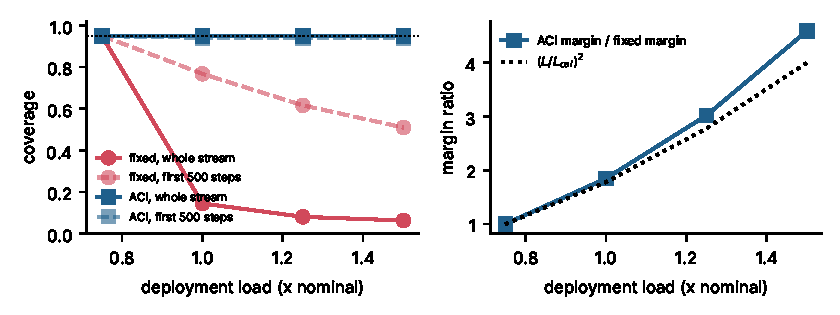
\includegraphics[width=.85\linewidth]{figs/fig_conformal_shift.pdf}\caption{Coverage under load shift (left; solid: whole stream, dashed: first 500 steps; dotted line: target) and ACI margin relative to the fixed margin, with $(L/L_{\rm cal})^2$ for reference (right).}\label{fig:conf}\end{figure}
\textbf{Radial decomposition (remark).} For the exact branch-flow model on a tree, cutting branch $(i,j)$ makes the two sides depend on each other only through $\xi=(v_i^2,P_{ij},Q_{ij})$: given $\xi$, the downstream subtree is solved by a forward sweep from $v_j^2=v_i^2-2(r_{ij}P_{ij}+x_{ij}Q_{ij})+(r_{ij}^2+x_{ij}^2)(P_{ij}^2+Q_{ij}^2)/v_i^2$ and its own injections, and the upstream side sees the cut only as an extra load $(P_{ij},Q_{ij})$ at $i$; consistency is one scalar equation. This is a standard property of tree power flow; we verified it numerically on 27/27 IEEE-33 cuts. A consensus-ADMM projection built on it is exact (gap $10^{-7}$--$10^{-5}$) but not faster than a monolithic interior-point solve (several $n{=}123$ and all $n{=}400$ many-block instances did not converge in 400 iterations), so we make no scalability claim.

\section{Headroom-gated evaluation}\label{sec:head}
\textbf{Definition.} $H=(J_{\rm ref}-J_{\rm oracle})/J_{\rm ref}$ where $J_{\rm ref}$ is the cost of the best \emph{violation-free} fixed heuristic after tuning on training days only (EDF power cap, or the projected uncontrolled rule) and $J_{\rm oracle}$ a perfect-foresight LP on the same network rows. Under the LP model no causal violation-free policy can gain more than $H$ in expectation. The LP is not a bound on the true environment: it ignores the SoC-dependent efficiency curve, and a clairvoyant per-day choice among heuristics can beat it.\\
\textbf{A correction.} Our headroom script ran the rule named \texttt{safe\_uncontrolled} without the projection, so it violated the network on 60--75\% of stress days yet qualified as ``best heuristic''. Against it JPL appeared to have $H\approx$13--17\%. Counting only violation-free references (EDF caps only) gives 38\%, and with the \emph{projected} uncontrolled rule, now run on 20 real weekdays, $H=1.7\%$ (Table~\ref{tab:head}, Fig.~\ref{fig:head}). Caltech was unaffected because its best reference was already a violation-free cap. The conclusion that JPL is where learning should be tried first is reversed.
\begin{table}[h]\centering\small
\begin{tabular}{@{}lcccc@{}}\toprule & \multicolumn{2}{c}{Caltech} & \multicolumn{2}{c}{JPL}\\ Price source & $H$ (\%) & clairv. $H$ (\%) & $H$ (\%) & clairv. $H$ (\%)\\\midrule
SCE TOU stand-in & 5.2 & 4.5 & 1.7 & 3.3\\
CAISO hourly (WEP) & 7.7 & 6.4 & 4.1 & 4.5\\
SCE TOU-EV-4 incl.\ demand charge & $-0.4^\dagger$ & 2.3 & $-7.4^\dagger$ & 2.8\\\bottomrule
\end{tabular}\caption{Headroom on 20 real weekdays (stress), projected violation-free references. ``clairv.'' uses the per-day best heuristic instead of the train-tuned one. $^\dagger$The LP returned ``solution may be inaccurate'' warnings and its value exceeds the best heuristic, so $H$ is not meaningful there. We did not diagnose the cause; two untested candidates are the long constant-price blocks of this tariff (degenerate LP) and the LP's omission of the SoC-dependent efficiency.}\label{tab:head}\end{table}
Earlier 8-day synthetic scenarios gave 7.3--8.2\% at Caltech for duck, volatile, solar-glut and flat prices; with real sources the range is wider (5.2--7.7\%), so we no longer claim that headroom is insensitive to price. At JPL the best reference is the projected uncontrolled rule in all sources, and headroom is at most 4.5\%.
\begin{figure}[h]\centering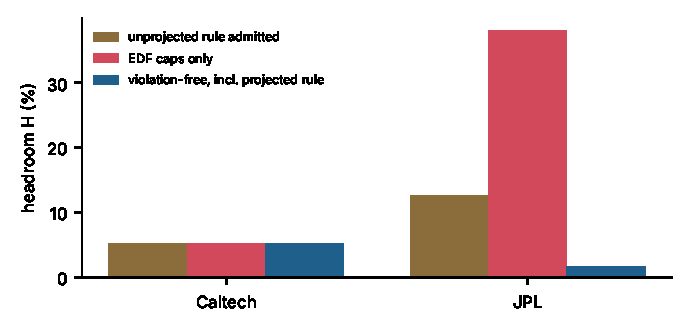
\includegraphics[width=.6\linewidth]{figs/fig_headroom_gating.pdf}\caption{Headroom (SCE TOU stand-in, 20 real weekdays) under three admission rules for the reference.}\label{fig:head}\end{figure}
\textbf{Sample size.} For paired daily differences with standard deviation $\sigma_\Delta$ and true mean gain $\mu$, the usual normal-approximation test needs $N\gtrsim(z_{1-\delta/2}+z_{\beta})^2\sigma_\Delta^2/\mu^2$ days. Since $\mu\le H J_{\rm ref}$ under the LP model, $N$ grows at least as $H^{-2}$ for fixed $\sigma_\Delta$. A Hoeffding gate is far more conservative (over 1000 days for a \$20/day gain), so deployment gates should use bootstrap or empirical-Bernstein bounds. We state this as a planning heuristic, not a theorem: $\sigma_\Delta$ also depends on the policy.

\section{Critic-based RL around a tuned rule}\label{sec:rl}
SafeTD3 is trained as a residual around the tuned EDF cap (action $=$ rule $+$ scaled correction, through the QP), with dense potential-based shaping~\cite{ng}, behaviour-cloning pre-training and best-versus-last checkpoint selection. On real Caltech held-out days over 3 seeds the cost relative to the tuned cap is $+6.3$, $+4.4$, $+8.5\%$ at residual scale 0.3 and $+1.8\%$ at 0.1; plain (non-residual) TD3 is $+41\%$. Regret is monotone in the allowed deviation, there are no violations, and lower exploration noise, Optuna-tuned hyperparameters and removing the conformal margin do not change the sign. On the synthetic stress days of Sec.~\ref{sec:twin} (where $H=33\%$) the same residual TD3 trained for 120 episodes (one seed, each episode a fresh synthetic day) is $+13.6\%$ worse than the tuned cap (1030 vs 907), so the failure is not explained by low headroom alone; we cannot exclude that a larger budget or different tuning would change this.

\section{A differentiable twin and pathwise policy learning}\label{sec:twin}
\textbf{Construction.} Admission and departure depend on time only, so given the exogenous day the cost is an almost-everywhere differentiable function of the action sequence: SoC dynamics with state-dependent efficiency, energy cost, unmet energy at departure, the day-peak demand charge and the LinDistFlow rows, written in PyTorch. A differentiable restoration step scales actions into $\{Gp\le h\}$: either uniformly, $p\leftarrow\alpha p$ with $\alpha=\min(1,\min_i h_i/(Gp)_i)$, or ``sens'': each violated row scales only the chargers with $G_{ik}>0$, followed by the uniform step to guarantee feasibility (rows can have mixed signs; the upstream-charger-unaffected property holds for thermal rows but not for voltage rows). An optional straight-through estimator keeps the exact max/min in the forward pass and uses a log-sum-exp gradient in the backward pass. Not differentiable: the AC solve (used only for evaluation), arrivals and departures, and degradation and discomfort terms (V2G off).\\
\textbf{Verification.} For identical random actions the twin and the simulator agree to $3.5\times10^{-16}$ relative cost on 10 synthetic days and $2\times10^{-16}$ on 10 real days, with no violations. Autograd versus central differences on 60 non-zero-gradient coordinates: median relative error $3\times10^{-7}$ (synthetic), $1.3\times10^{-4}$ (Caltech), $1.7\times10^{-6}$ (JPL); 77\%, 50\%, 67\% of coordinates agree to $10^{-4}$, the rest lie at $\max$/clip kinks.\\
\textbf{Experiment.} A causal shared MLP (10 per-slot features: price level and rank, SoC, deficit, time left, urgency, rating, site load, running peak; it sees the day's price vector, as the heuristics do) is trained on 30 days by backpropagating the cost through the 96- or 192-step rollout, with no critic, and evaluated in the real simulator on 20 held-out days. Table~\ref{tab:twin} and Fig.~\ref{fig:twin} give the results.
\begin{table}[h]\centering\small
\resizebox{\linewidth}{!}{\begin{tabular}{@{}llcccc@{}}\toprule Days & Headroom & tuned ref & residual TD3 & pathwise (3 seeds) & LP oracle\\\midrule
Synthetic stress & 32.7\% & 906.7 & 1030.2 & 779.7/783.2/780.9 (uniform) & 610.0\\
 & & & & 815.2/820.0/817.0 (sens+STE) & \\
Real Caltech & 6.2\% & 386.1 & --- (Sec.~\ref{sec:rl}) & 386.7/386.5/418.8 (sens+STE) & 362.2\\
Real JPL & 0.7\% & 754.5 & --- & 857.1/889.3/889.3 (uniform); 829.0 (sens+STE, 1 seed) & 748.9\\\bottomrule
\end{tabular}}\caption{Mean cost per day on 20 held-out days (30 training days; random split). Real-day runs use the SCE TOU stand-in price. The headroom printed here is computed on these 20 held-out days and therefore differs from Table~\ref{tab:head}, which uses 20 evenly spaced weekdays. The uniform variant was not run on real Caltech days and the sens+STE variant on JPL completed one seed.}\label{tab:twin}\end{table}
\begin{figure}[h]\centering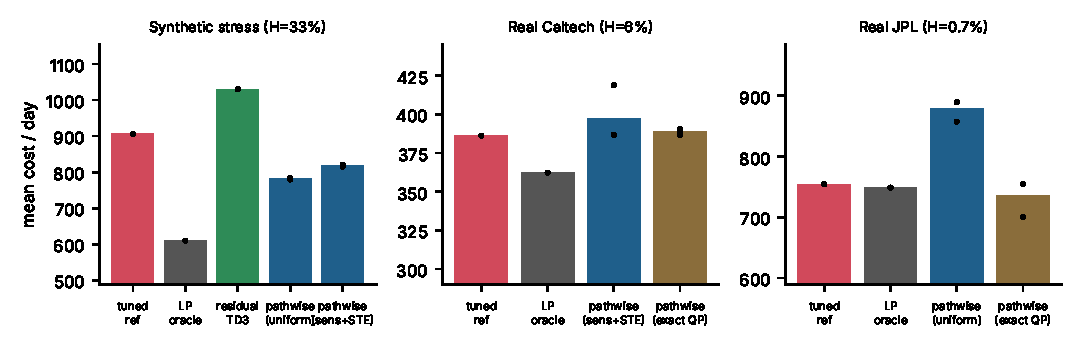
\includegraphics[width=\linewidth]{figs/fig_diffenv_poc.pdf}\caption{Held-out mean cost; dots are individual seeds. ``Exact QP'' bars are the retrained networks of Sec.~\ref{sec:pp} run live under the exact QP projection (Table~\ref{tab:pp}); the other pathwise bars use the twin's ray-scaling restoration, and come from earlier runs with slightly different seeds.}\label{fig:twin}\end{figure}
\textbf{Reading.} At 33\% headroom pathwise learning beats the tuned cap by 10--14\% with no violations, and also beats the clairvoyant per-day best cap (834.7), closing about 42\% of the LP gap. At 6\% headroom (Caltech) it matches the reference (+0.1\%, +0.2\%, +8.5\%; the first seed's paired bootstrap CI includes zero), and at JPL (0.7\%) the first run looked 10--18\% worse with 85--87\% of energy served. Section~\ref{sec:pp} shows that this is caused by the restoration step, not by the policy. Two changes (headroom and gradient access) coincide in the synthetic comparison with TD3, so we do not attribute the difference to either one. A cleaner test requires the same method on a high-headroom \emph{real} regime, which we did not find.\\

\textbf{The projection price (closed loop).}\label{sec:pp} The restoration used inside the twin (uniform ray scaling) differs from the exact QP projection the reference uses. To separate the two we ran the same trained network \emph{live} in the simulator under each projection, using the 20 held-out days of Table~\ref{tab:twin} (retrained, 300 iterations; \texttt{proj\_price\_closed\_loop.py}). Two checks validate the plumbing: the rule ``charge at full rate'' under the QP equals the tuned reference at JPL (754.5), and each network under ray scaling in the simulator reproduces its twin cost (e.g.\ 847.9 vs 848.1).
\begin{table}[h]\centering\small\begin{tabular}{lcccc}
JPL & cost, ray scaling & served & cost, exact QP & served\\\hline
full-rate rule (= tuned reference under QP) & 889.3 & 0.855 & 754.5 & 0.921\\
pathwise, seed 0 & 847.9 & 0.868 & 700.3 & 0.924\\
pathwise, seeds 1, 2 & 889.3 & 0.855 & 754.5 & 0.921\\
safe initial action (0.27 of max), seed 0$^\ddagger$ & 889.3 & 0.855 & 754.5 & 0.921\\
sens+STE, safe initial action, seeds 0--2 & 870.4 & 0.862 & 754.5 & 0.921\\\hline
Caltech (tuned cap reference 386.1) & & & &\\
pathwise, seeds 0 / 1 / 2 & 386.5 / 385.4 / 386.8 & 0.81 & 388.7 / 386.7 / 390.3 & 0.81
\end{tabular}\caption{Held-out cost per day (20 days; no constraint violations in any run). The cost of the same actions depends on the projection. $^\ddagger$One seed only (run stopped).}\label{tab:pp}\end{table}
At JPL, replacing the QP by ray scaling raises the reference rule's cost by 17.9\%. Seed 0 under the exact QP costs 700.3, 7.2\% below the reference (paired bootstrap 95\% CI $-75$ to $-33$ per day; better on 16 of 20 days). Seeds 1 and 2 never left their initialisation (training cost constant), so they equal the rule. We tried two remedies. Starting the policy at 0.27 of the maximum rate (strictly inside the feasible set) did not help: the one seed we ran climbed back to full rate within 100 iterations and stopped at the same plateau (training cost 956.1). Training with the sens+STE backward pass and the same safe start also ended on the full-rate plateau in all three seeds (twin cost 870.4, equal to the full-rate rule's own cost under that restoration, hence 754.5 under the QP). Counting every run, one of seven attempts escaped the plateau. A plausible but untested explanation is that ray scaling is homogeneous of degree zero, so on steps where a row binds the cost does not depend on the overall scale of the action and the gradient along it vanishes, while a saturated sigmoid adds a second flat region; a restoration that is not scale-invariant (an unrolled QP projection) would be the natural next test, which we did not run. The seed-0 policy's cost is below the LP oracle's 748.9, so the LP is not a lower bound under this cost (it ignores the SoC-dependent efficiency), and the JPL headroom of 0.7\% is probably an underestimate. At Caltech the projection makes no practical difference and the policy matches the reference. One seed learning at one site is a pilot result, not a finding.

\textbf{Chronological pre-COVID split.} To remove the random-split and 2020-lockdown caveats we repeated the twin experiment on 2019 only: 30 weekdays from 1 Jan to 2 Aug for training and tuning, and the 20 following weekdays (9 Aug--31 Dec) for testing, three seeds, 300 iterations, uniform restoration.
\begin{table}[h]\centering\small\begin{tabular}{lccccc}
2019 split & headroom & reference & LP oracle & pathwise (3 seeds) & served\\\hline
Caltech & 5.0\% & 320.5 (cap 0.6) & 304.4 & 365.7 / 365.7 / 365.7 & 0.89\\
JPL & $-0.7$\% & 969.1 (projected full rate) & 975.6 & 1195.0 / 1122.7 / 1121.8 & 0.78--0.81
\end{tabular}\caption{Held-out cost per day on the chronological split; no constraint violations in any run.}\label{tab:chrono}\end{table}
Here pathwise learning is 14\% (Caltech) and 16--23\% (JPL) worse than the reference. At Caltech the three seeds are identical and equal to the full-rate rule: the training cost never moved from its initial plateau, so no learning occurred, and the random-split result that pathwise ``matches'' the reference (Table~\ref{tab:twin}) does not carry over, because there the tuned cap was close to full rate. We did not run the exact-QP closed-loop evaluation on this split, so we cannot say how much of the JPL gap is the restoration step as in Sec.~\ref{sec:pp}. The headroom is similar to the random-split numbers (5.0\% against 6.2\% at Caltech) and the LP is again no better than the reference at JPL.
\textbf{Planning versus learning.} With perfect foresight, open-loop Adam on the twin reaches 795 (uniform) and 708 (sens+STE) on the synthetic days against 610 for the LP: plain gradient descent on this piecewise-linear problem is a poor planner, and spreading the backward pass of the peak and the restoration over near-active entries helps (795$\to$708) without closing the gap. A learned causal policy (781) beat the 300-iteration open-loop planner (795). We did not isolate why; the planner's subgradient is concentrated on a single peak step and a single binding row, which is a plausible but untested explanation, and sens+STE did not improve the learned policy (815--820 vs 780), so the variants are not uniformly better.


\section{The residual world model}\label{sec:wm}
The original design predicts the next state as $\hat s_{t+1}=F_{\rm base}(s_t,a_t)+N_\theta(s_t,a_t)$, with $F_{\rm base}$ the LinDistFlow/SoC model and $N_\theta$ a small network (output scaled to a few percent of the range, initialised near zero, with an exact-KVL penalty). We ran the first planned ablation, on synthetic stress days, with targets from the exact AC solve and episodes split by day (up to 2880 training and 960 held-out transitions; three seeds; 1500 steps): $F_{\rm base}$ only, $F_{\rm base}+N_\theta$, and a black-box network (hidden width 256, depth 3) with no physics prior.
\begin{table}[h]\centering\small\begin{tabular}{lcccc}
Model & voltage MAE & voltage max err & branch-$S$ MAE & SoC MAE\\\hline
$F_{\rm base}$ only & $2.1\times10^{-4}$ & $5.5\times10^{-3}$ & $6.4\times10^{-3}$ & 0.024\\
$+N_\theta$ (100 / 2880 samples) & $2.7$ / $1.8\times10^{-4}$ & $6.0$ / $2.0\times10^{-3}$ & $3.0$ / $2.1\times10^{-3}$ & 0.031 / 0.048\\
black-box (100 / 2880) & $1.5\times10^{-2}$ / $1.6\times10^{-2}$ & 0.16 / 0.20 & 0.046 / 0.045 & 0.14 / 0.083
\end{tabular}\caption{One-step prediction error on held-out synthetic days (p.u. except SoC). Means of 3 seeds; $F_{\rm base}$ is deterministic.}\label{tab:wm}\end{table}
Without a physics prior the network is about 70 times worse in voltage at every size we tried, so the analytic base is what carries accuracy. The residual improves the worst-case voltage error by 2.8$\times$ and branch flows by 3$\times$ once it has about a thousand transitions, but the mean voltage error improves only by 15\%, and it makes the SoC prediction \emph{worse} (0.024 to 0.048).

\textbf{The SoC regression is explained.} A follow-up on the same data (3 seeds, 2880 training and 960 held-out transitions; \texttt{wm\_ablation2.py}) splits SoC error into slots that stay occupied through the step and slots at an arrival or departure. $F_{\rm base}$ has SoC error $1.1\times10^{-4}$ on continuous slots (97\% of occupied slots); the 0.024 headline comes entirely from the 3\% boundary steps, where SoC resets or jumps and no dynamics model applies. The residual's SoC head, trained on those boundary steps, raises the continuous-slot error to 0.025, a 200-fold regression. Removing the SoC head (grid residual only) restores $1.1\times10^{-4}$; a per-slot shared network for $\Delta$SoC changes nothing because $F_{\rm base}$ is already near-exact there. We therefore use $N_\theta$ for voltage and flow only.

\textbf{It shrinks the conformal margin.} With empirical margins calibrated on the first half of the held-out days and checked on the second half (one-step error against the exact AC solve):
\begin{table}[h]\centering\small\begin{tabular}{lcccc}
Model & $\tau_v$ (5\%) & $\tau_v$ (1\%) & $\tau_S$ (1\%, rating-norm.) & test coverage (v, S)\\\hline
$F_{\rm base}$ only & $1.95\times10^{-3}$ & $2.97\times10^{-3}$ & $1.52\times10^{-2}$ & 0.983, 0.985\\
$+N_\theta$ with SoC head & $1.29\times10^{-3}$ & $1.41\times10^{-3}$ & $9.5\times10^{-3}$ & 0.956, 0.986\\
$+N_\theta$ grid only & $1.13\times10^{-3}$ & $1.14\times10^{-3}$ & $1.6\times10^{-3}$ & 0.989, 0.991\\
black-box & $8.3\times10^{-2}$ & $1.1\times10^{-1}$ & $1.6\times10^{-1}$ & 0.968, 0.995
\end{tabular}\caption{Required safety margins (p.u.; $\tau_S$ as a fraction of the branch rating, under-prediction only) at 1\% and 5\% levels, and coverage at the 1\% level on the held-out half. Synthetic days; 3 seeds.}\label{tab:wm2}\end{table}
The grid-only residual cuts the 1\% voltage margin 2.6$\times$ and the rating-normalised branch margin 9.8$\times$, with coverage at about the 0.99 target. The mean error understated this: margins are set by the tail. Scope: synthetic days, one-step prediction, hub-level loads; we have not tested the effect on policy cost (ablation A5 proper) or on real days, and the other three planned ablations (safety layer, federated, willingness) are implemented but not run for this draft.


\section{Bidirectional V2G: what we measured}\label{sec:v2g}
The headline runs are unidirectional. We checked what discharge would add on 8 synthetic days at normal load with the SCE TOU stand-in price (\texttt{v2g\_discharge\_check.py}; per-direction efficiency 0.95 with a quadratic taper, i.e.\ about 0.90 round trip, a degradation term, and the \$2/kWh unmet penalty; the plans are executed in the simulator, so all costs are simulator costs). The hindsight LP oracle with discharge is cheaper than without by \$57.2 per day on average (15.4\%; positive on all 8 days, \$19--88), while the causal rule \texttt{v2g\_greedy} is 16.0\% \emph{more} expensive than the non-discharging TOU rule. So discharge is worth a lot to a clairvoyant planner and nothing to a naive causal one. An earlier, collaborator-reported four-arm study (a synthetic CAISO-like price) found an oracle gain of at most \$0.9/day and naive V2G 26--52\% worse; we did not reproduce the first number under our price and battery assumptions, and we did not re-run that study. We therefore do not claim that V2G profit is negligible; we leave it out of the main comparison because the causal baselines lose with it, and because ACN sessions have short dwell times that we have not analysed for V2G potential. This is untested territory and a candidate high-headroom regime for learned policies.

\section{Relation to the original proposal}
Ideas from the proposal and what became of them: the analytic-plus-residual world model (Sec.~\ref{sec:wm}: the voltage/flow residual cuts the required conformal margin 2.6--9.8$\times$ in one-step tests; its SoC head hurts and was removed); the differentiable QP safety layer (used throughout as the projection; the soft-penalty comparison is implemented, not run here); conformal margin tightening (Sec.~\ref{sec:conf}: extended to row-wise, joint-coverage and online versions, which the proposal did not have); personalised federated learning (pilot: no benefit over local tuning); willingness-aware bidding and V2G discharge (V2G discharge disabled in the headline runs, see below; willingness ablation not run); scaling to the 123-bus feeder (the tree-decomposition lemma was checked on 123-bus cuts, but the decomposed solver was not faster). Added during the study and not in the proposal: the headroom gate, the differentiable twin and pathwise learning, and the load-shift conformal analysis.

\section{Limitations}
Balanced single-phase network and an AC reference that shares the model; one feeder; two sites; one random 30/20 split per site plus one chronological 2019 split (train Jan--Aug, test Aug--Dec), 3 seeds each; wholesale price is a system-level series and the tariff schedule is applied to both sites by assumption; the LP oracle is unreliable under the tariff source and can be beaten by clairvoyant heuristics; no forecast-aware MPC baseline (ours has no arrival forecast and was worse than the tuned cap); the TD3 comparison on synthetic days is one seed and 120 episodes; the world-model results use synthetic days and one-step errors only; federated averaging showed no benefit over local tuning in a two-site pilot; no guarantee for joint multi-step safety. We make no claim of ``guaranteed zero violations'': zero were observed, and the conformal statements hold under their stated assumptions.

\section{Reproducibility}
\sloppy Code, result files and a SHA-256 manifest are in the accompanying repository (\texttt{REPRODUCE.md}, \texttt{docs/PAPER\_COMMANDS.md}); versions are pinned, CPU runs are bit-exact, CUDA runs are not. Figures are generated from the result files by \texttt{scripts/make\_paper\_figs.py}. Key scripts: \texttt{adaptive\_conformal\_shift.py}, \texttt{conformal\_normalised\_shift.py}, \texttt{conformal\_rowwise\_vs\_global.py}, \texttt{headroom\_multiday.py}, \texttt{diff\_env\_poc.py}, \texttt{td3\_synth\_stress.py}, \texttt{wm\_ablation.py}, \texttt{wm\_ablation2.py}; the one-command Windows runner is \texttt{RUN\_ALL.ps1}; tests in \texttt{tests/test\_diffenv.py}.

\section{Conclusion}
The defensible results are about safety calibration (what fixed margins lose under shift, why the needed margin is physical, and why joint coverage needs Bonferroni or a normalised score) and about evaluation (headroom against a tuned, violation-free reference, with the correction above). On the real Caltech and JPL days we tested (a random and a chronological 2019 split), the oracle-based headroom is 2--8\%; critic-based learning did not beat the tuned heuristic, pathwise learning matched it at Caltech on the random split and was 14\% worse on the chronological split (where it did not learn), and at JPL one of seven runs beat it by 7\% once the learned actions were projected exactly (the other six stayed at the reference rule), which shows that the LP-based headroom can understate what is achievable there but that the gain is not robust. Pathwise gradients through a verified twin do win where headroom is large, but only on synthetic days. Next steps: find or construct a real high-headroom regime, add TD3/SAC/Lagrangian/PI-TD3 baselines on the same days, test model mismatch against an unbalanced three-phase model, and run 40--60 test days with 5 seeds.

\begin{thebibliography}{99}\small
\bibitem{ev2gym} S.~Orfanoudakis, C.~Diaz-Londono, Y.~E.~Y{\i}lmaz, P.~Palensky, P.~P.~Vergara. EV2Gym: A flexible V2G simulator for EV smart charging research and benchmarking. \emph{IEEE Trans.\ Intelligent Transportation Systems} 26(2):2410--2421, 2025.
\bibitem{pitd3} S.~Orfanoudakis, F.~A.~Oliehoek, P.~Palensky, P.~P.~Vergara. Physics-informed reinforcement learning for large-scale EV smart charging considering distribution network voltage constraints. arXiv:2510.12335.
\bibitem{tlmappo} C.~Huang, J.~Fan, W.~Wang, H.~Wang. Safe decentralized operation of EV virtual power plant with limited network visibility via multi-agent reinforcement learning. arXiv:2604.03278.
\bibitem{optnet} B.~Amos, J.~Z.~Kolter. OptNet: Differentiable optimization as a layer in neural networks. ICML 2017.
\bibitem{cvxpylayers} A.~Agrawal, B.~Amos, S.~Barratt, S.~Boyd, S.~Diamond, J.~Z.~Kolter. Differentiable convex optimization layers. NeurIPS 2019.
\bibitem{dalal} G.~Dalal, K.~Dvijotham, M.~Vecerik, T.~Hester, C.~Paduraru, Y.~Tassa. Safe exploration in continuous action spaces. arXiv:1801.08757, 2018.
\bibitem{vovk} V.~Vovk, A.~Gammerman, G.~Shafer. \emph{Algorithmic Learning in a Random World}. Springer, 2005.
\bibitem{lei} J.~Lei, M.~G'Sell, A.~Rinaldo, R.~J.~Tibshirani, L.~Wasserman. Distribution-free predictive inference for regression. \emph{J.\ Am.\ Stat.\ Assoc.} 113(523), 2018.
\bibitem{aci} I.~Gibbs, E.~J.~Cand\`es. Adaptive conformal inference under distribution shift. NeurIPS 2021.
\bibitem{acofi} S.~Huriot, I.~Tabbara, H.~Sibai. Safe control using learned safety filters and adaptive conformal inference. arXiv:2604.18482.
\bibitem{zapico} D.~Fern\'andez-Zapico, T.~Hofman, M.~Salazar. Stochastic model predictive control of charging energy hubs with conformal prediction. arXiv:2504.00685.
\bibitem{ruddick} J.~Ruddick, G.~Ceusters, G.~Van~Kriekinge, E.~Genov, C.~De~Cauwer, T.~Coosemans, M.~Messagie. Real-world validation of safe reinforcement learning, model predictive control and decision tree-based home energy management systems. arXiv:2408.07435.
\bibitem{henderson} P.~Henderson, R.~Islam, P.~Bachman, J.~Pineau, D.~Precup, D.~Meger. Deep reinforcement learning that matters. AAAI 2018.
\bibitem{precipice} R.~Agarwal, M.~Schwarzer, P.~S.~Castro, A.~Courville, M.~G.~Bellemare. Deep reinforcement learning at the edge of the statistical precipice. NeurIPS 2021.
\bibitem{shac} J.~Xu, V.~Makoviychuk, Y.~Narang, F.~Ramos, W.~Matusik, A.~Garg, M.~Macklin. Accelerated policy learning with parallel differentiable simulation. ICLR 2022 (arXiv:2204.07137).
\bibitem{dpf} M.~\"Oz, J.~H\"orter, K.~Phipps, C.~Debus, A.~Streit, M.~G\"otz. Differentiable power-flow optimization. arXiv:2603.28203.
\bibitem{distev} A.~Ghavami, K.~Kar, A.~Gupta. Decentralized charging of plug-in electric vehicles with distribution feeder overload control. arXiv:1308.4316.
\bibitem{boyd} S.~Boyd, N.~Parikh, E.~Chu, B.~Peleato, J.~Eckstein. Distributed optimization and statistical learning via the alternating direction method of multipliers. \emph{Found.\ Trends Mach.\ Learn.} 3(1), 2011.
\bibitem{baranwu} M.~E.~Baran, F.~F.~Wu. Network reconfiguration in distribution systems for loss reduction and load balancing. \emph{IEEE Trans.\ Power Delivery} 4(2):1401--1407, 1989.
\bibitem{acn} Z.~J.~Lee, T.~Li, S.~H.~Low. ACN-Data: Analysis and applications of an open EV charging dataset. ACM e-Energy 2019.
\bibitem{wep} D.~Millstein, E.~O'Shaughnessy, R.~Wiser. Wholesale Electricity Prices (WEP) tool. Lawrence Berkeley National Laboratory, 2026.
\bibitem{ng} A.~Y.~Ng, D.~Harada, S.~Russell. Policy invariance under reward transformations: theory and application to reward shaping. ICML 1999.
\end{thebibliography}
\end{document}
